\documentclass{ximera}
\begin{document}

\subsection{Curve Sketching}
\subsubsection{Introduction}
\begin{dialogue}
\speak{Dylan} Using CAS systems to graph is great and all, but on a test where I don't have a calculator it's so hard to sketch a curve!
\speak{James} Well maybe we can use derivatives to figure out properties of the graph so it's easier to sketch!
\speak{Dylan} Oh! We'd be able to see where the graph was heading up or down, plus we'd be able to see maxima when the derivative at a point is zero!
\end{dialogue}
\subsubsection{Guided Problems}
Using your favorite computer algebra system, answer the following questions. Include an image of your graphs along with your answers, so the instructor may see your progress in your lab submission. 

\begin{enumerate}
\item{Graph the function $f(x)=x^3+12x^2+4$.}
\begin{enumerate}
\item{Indicate the intervals which have positive and negative slopes, and indicate the locations at which the slope changes sign. At these points, please indicate if the slope is changing from positive to negative or negative to positive. What do you expect the derivate to be at these points?}
\item{Using your CAS, determine the derivative of the given function. Then, evaluate the derivative at the points you indicated, as well as a point on each interval you indicated. Were you correct in your prediction in (a)? What can you predict about a graph at a point where the derivative is 0?}
\item{Create a number line, and mark the points where derivative was zero. Between these points, mark the sign of the derivative of any point on that interval.(You may do this by hand as it is difficult to format using most CAS systems) What do you notice? What can we say about a point with a derivative of zero when the sign changes from positive to negative? What about negative to positive?}
\end{enumerate}

\begin{dialogue}
\speak{Julia} So we have local maxima and minima when the derivative is 0, but what about the graph of $x^3$? 
\end{dialogue}
\begin{center}
\begin{tikzpicture}
  \begin{axis}[axis lines=center]
  \addplot [mark=none] {x^3};
\end{axis}
\end{tikzpicture}
\end{center}
\begin{dialogue}
\speak{Dylan} Hmmm...I guess that means there are three different kinds of critical points! Two when the sign changes and one when it stays the same!
\speak{Julia} Wait... what's a critical point?
\speak{Dylan} Any point where the derivative is zero or does not exist! Because we know it's important, but we have to check to see what it means with our number line!
\speak{James} You guys are still figuring that out? I'm already determining concavity!
\speak{Dylan and Julia} Holy cat fur! What's concavity?!
\speak{James} A graph is \textit{concave up when its derivative is increasing}, and \textit{concave down when its derivative is decreasing}. The easiest way to tell is to look at the curve and think `Would this hold water?' If it would, it's concave up, and if not, it's concave down!
\speak{Dylan and Julia} Wow! Thanks James!
\end{dialogue}
\begin{enumerate}
\item{Examine the graph of the original function. Note where this graph is concave up and concave down.}
\item{Examine the graph of the derivative. Note where this graph is increasing and decreasing.}
\item{What is happening on the graph of the function at the point where its derivative is at its minimum? What might this mean in general for extrema of a derivative?}
\item{Now use your CAS to determine the derivative of the function's derivative, $f''(x)$. Then evaluate at interesting points on the graph of the derivative. What is happening when the second derivative is zero? These points are known as inflection points.}
\item{Draw another number line, this time for the second derivative, marking the inflection points. Evaluate $f''(x)$ on a point of each of the intervals created through this marking, and mark the sign. What might this mean in general for changing signs on each side of an inflection point?}
\item{Inflection points are given as ordered pairs. Evaluate each inflection point you found using $f(x)$ to determine the ordered pairs.}
\end{enumerate}
\end{enumerate}
\subsubsection{Matching Graphs}
\begin{dialogue}
\speak{Dylan}So if I wanted to match a graph with the graphs of its first and second derivative I can do that now!
\speak{Julia} Wait, really?? How?
\speak{James} Well the $y$ value of $f'(x)$ corresponds to the slope of $f(x)$, and the $y$ value of $f''(x)$ corresponds to the slope of $f'(x)$ and is related to the concavity of $f(x)$
\speak{Julia} So we can match the graphs based on how all that information relates!
\speak{Dylan} Exactly, let's try it!
\end{dialogue}
Match each graph to its first and second derivative, create a table to organize by $f(x),f'(x)$, and $f''(x)$.
\begin{figure}[h]
    \centering
    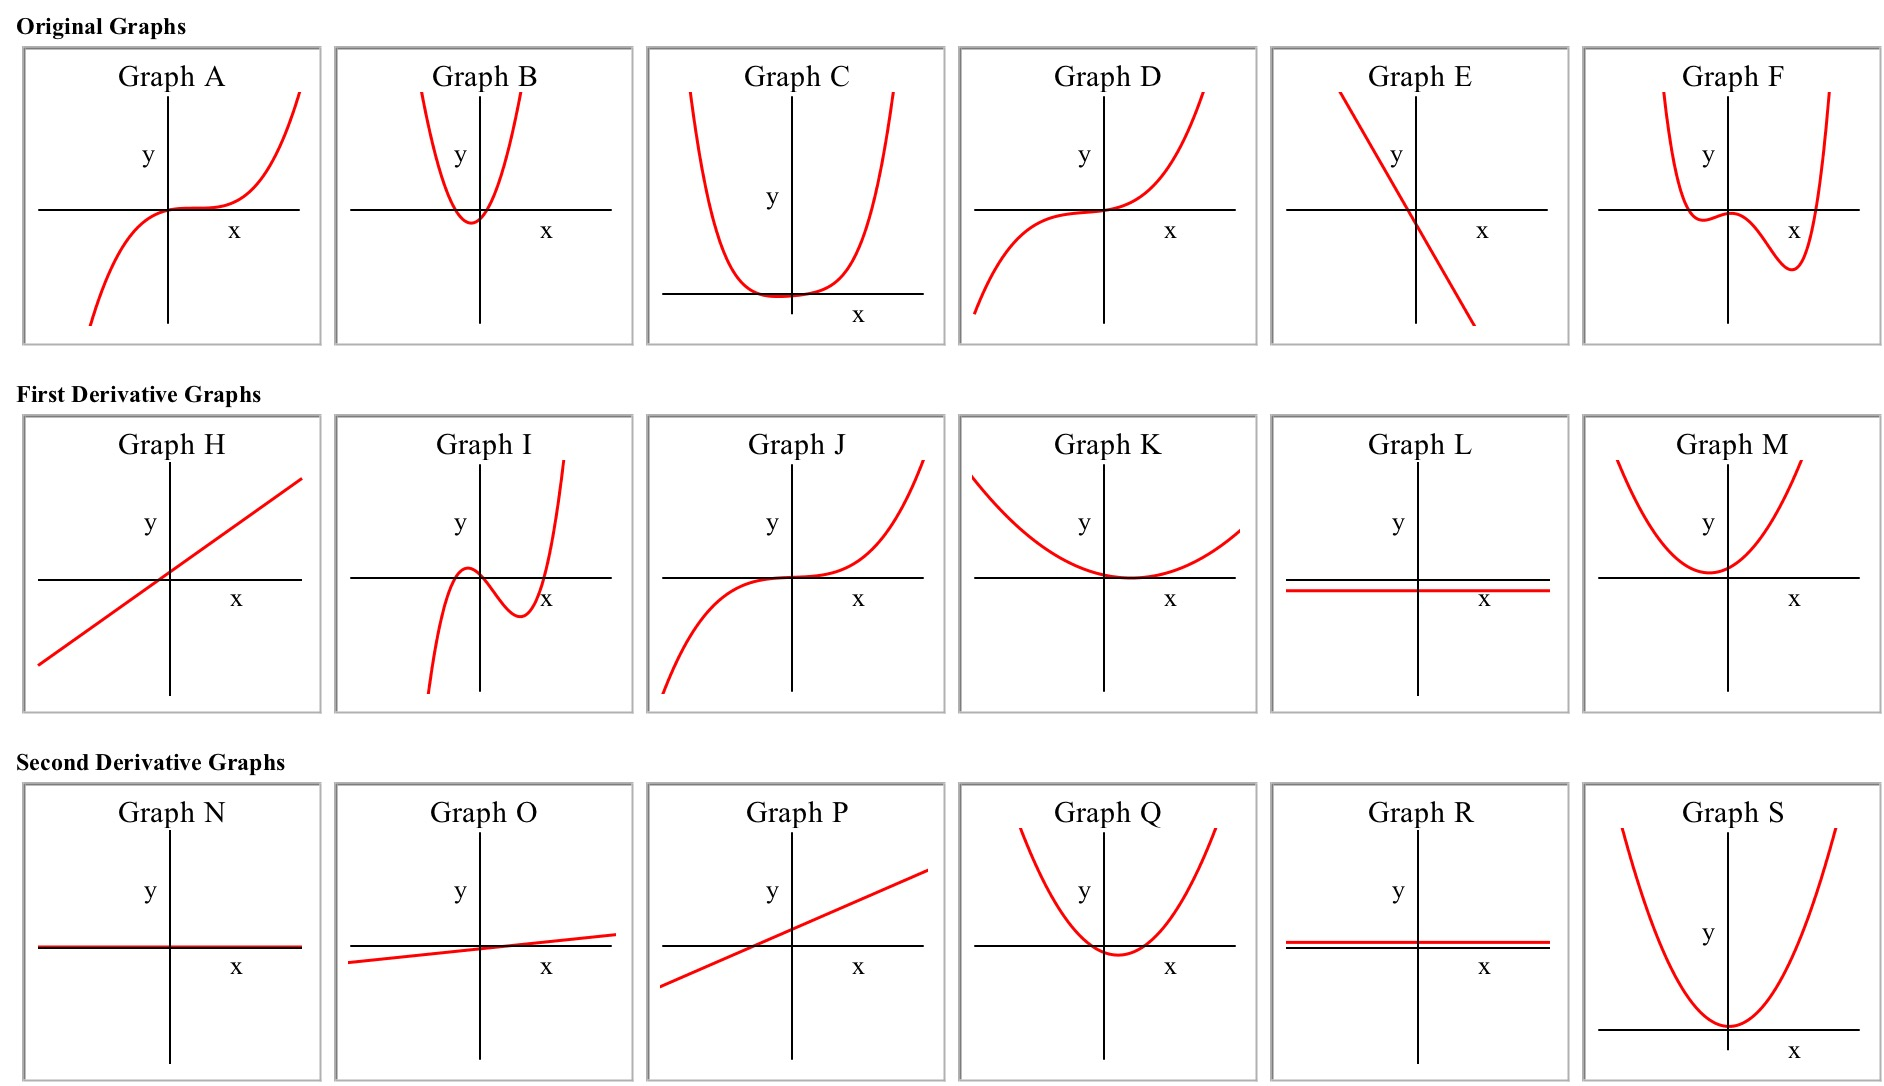
\includegraphics[width=150mm]{matching.jpg}
    \label{fig:matching}
\end{figure}

\subsubsection{On Your Own}
Now, for the function $$x^5-5x^4+5x^3+5x^2-6x-1$$. Find:
\begin{itemize}
\item{Extrema}
\item{Critical Points}
\item{Inflection Points}
\item{Concavity}
\end{itemize}


\subsubsection{In Summary}
In this lab, you've covered quite a bit. To help organize everything, we've made the following table for you.

\begin{center}
    \begin{tabular}{| l | p{7.5cm} |}
    \hline
    First Derivative Test & When $f'(x) = 0$: \begin{enumerate}
    \item{A maximum occurs if at this point, the sign of the derivative changes from positive to negative.}
    \item{A minimum occurs at this point if the sign of the derivative changes from negative to positive.}
    \item{An inflection point occurs at this point if the sign of the derivative stays the same.}
    \end{enumerate}
    \item{When $f'(x)$ does not exist\:}
    \begin{enumerate}
    \item{If x is in the domain of $f(x)$, follow the same steps as when $f'(x)=0$}
    \item{If x is not in the domain, then it is a critical point but not a maximum, minimum, or inflection point (ex.asymptote)}
    \end{enumerate}\\
    \hline
    Second Derivative Test &  At a critical point: \begin{enumerate}
    \item{A local maximum occurs if $f''(x)>0$.}
    \item{A local minimum occurs if $f''(x)<0$.}
    \item{The test fails if $f''(x)=0$.}
    \end{enumerate}\\ \hline
    \end{tabular}
\end{center}
\end{document}
\pagebreak